\documentclass[a4paper, 11pt]{book}
\usepackage{/home/nicolas/Documents/Enseignement/Prepa/bpep/fichiers_utiles/preambule}

\newcommand{\dsNB}{16}
\makeatletter
\renewcommand{\@chapapp}{Kh\^olles MPSI3 -- semaine \dsNB}
\makeatother

% \toggletrue{corrige}  % décommenter pour passer en mode corrigé

% IMPORTS automatiques
\newcommand{\f}[2]{{
		\mathchoice
		{\dfrac{#1}{#2}}
		{\dfrac{#1}{#2}}
		{\frac{#1}{#2}}
		{\frac{#1}{#2}}
}}

\newcommand{\e}[1]{{}_{\text{#1}}}

 % fin des IMPORTS automatiques

\begin{document}

\chapter{Sujet 1\siCorrige{\!\!-- corrig\'e}}
\section{Question de cours}

Présenter les coordonnées cylindriques avec un schéma introduisant la base et
indiquant les coordonnées, donner l'expression de $\vv{\rm OM}$ dans cette base, donner
\textbf{et démontrer} l'expression de la vitesse, du déplacement élémentaire et
de l'accélération en coordonnées cylindriques.

\resetQ
\subimport{/home/nicolas/Documents/Enseignement/Prepa/bpep/exercices/TD/mesurer_masse_atronaute/}{sujet.tex}

\chapter{Sujet 2\siCorrige{\!\!-- corrig\'e}}
\section{Question de cours}

Présenter les lois du frottement de \textsc{Coulomb}, et refaire
l'exercice~:
\begin{NCexem}[width=\linewidth]{Plan incliné et frottements solides}
    \begin{minipage}{0.6\linewidth}
        On considère un plan incliné d'un angle $\alpha = \ang{20;;}$ par
        rapport à l'horizontale. Une brique de masse $m = \SI{600}{g}$ est
        lancée depuis le bas du plan vers le haut, avec une vitesse $v_0 =
        \SI{2.4}{m.s^{-1}}$. Pour étudier le mouvement, on utilise le repère
        (O,$x$,$y$) avec O coïncidant avec la position de départ de la brique.
        On note $g$ l'accélération de la pesanteur, avec $g =
        \SI{9.81}{m.s^{-2}}$. On suppose qu'il existe des frottements solides,
        avec $f$ le coefficient de frottements solides tel que $f =
        \num{0.20}$.\bigbreak
    \end{minipage}
    \hfill
    \begin{minipage}{0.35\linewidth}
        \begin{center}
            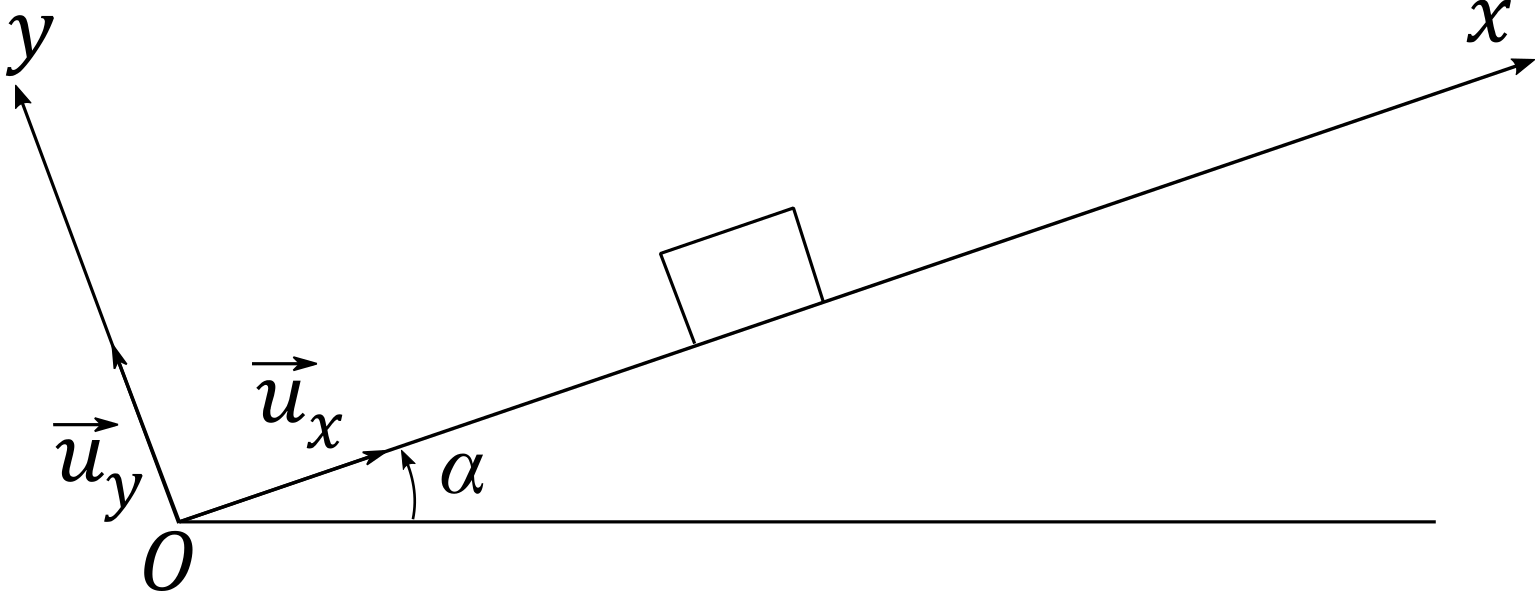
\includegraphics[width=\linewidth]{../../figures/ch16/plan_incl-plain}
        \end{center}
    \end{minipage}
    \begin{enumerate}
        \item Établir l'équation horaire du mouvement de la brique lors de
            sa montée.
        \item Déterminer la date à laquelle la brique s'arrête, ainsi que la
            distance qu'elle aura parcourue.
    \end{enumerate}
\end{NCexem}

\resetQ
\subimport{/home/nicolas/Documents/Enseignement/Prepa/bpep/exercices/TD/chute_de_bille/}{sujet.tex}


\chapter{Sujet 3\siCorrige{\!\!-- corrig\'e}}
\section{Question de cours}

Étude du pendule simple~: mise en situation, équation différentielle,
linéarisation, résolution.

\resetQ
\subimport{/home/nicolas/Documents/Enseignement/Prepa/bpep/exercices/TD/ski/}{sujet.tex}

\chapter{Sujet 4\siCorrige{\!\!-- corrig\'e}}
\section{Question de cours}

Énoncer les trois lois de \textsc{Newton}, définir le centre d'inertie d'un
ensemble de points, le vecteur quantité de mouvement d'un ensemble de points et
son lien avec le centre d'inertie, énoncer et démontrer le théorème de la
résultante cinétique.
    
\resetQ
\subimport{/home/nicolas/Documents/Enseignement/Prepa/bpep/exercices/TD/prob_ouverts_dynamique/}{sujet.tex}

\label{LastPage}
\end{document}
